\subsection{Descripci\'on del problema}



\subsection{Resoluci\'on}



%\subsection{Demostraci\'on de la resoluci\'on}


\subsection{Complejidad del algoritmo}


\subsection{C\'odigo fuente}

\lstset{language=C++,
                basicstyle=\ttfamily\footnotesize,
                keywordstyle=\color{blue}\ttfamily,
                stringstyle=\color{red}\ttfamily,
                commentstyle=\color{green}\ttfamily,
                morecomment=[l][\color{magenta}]{\#},
                breaklines=true
}
\begin{lstlisting}


\end{lstlisting}

\subsection{Casos de prueba}

Para este ejercicio escogimos algunos casos de prueba que tienen las siguientes características:

\begin{itemize}

\item 
\item 
\item 
\item 
\item 

\end{itemize}


\subsection{Performance}



\begin{figure}[H]
\begin{center}
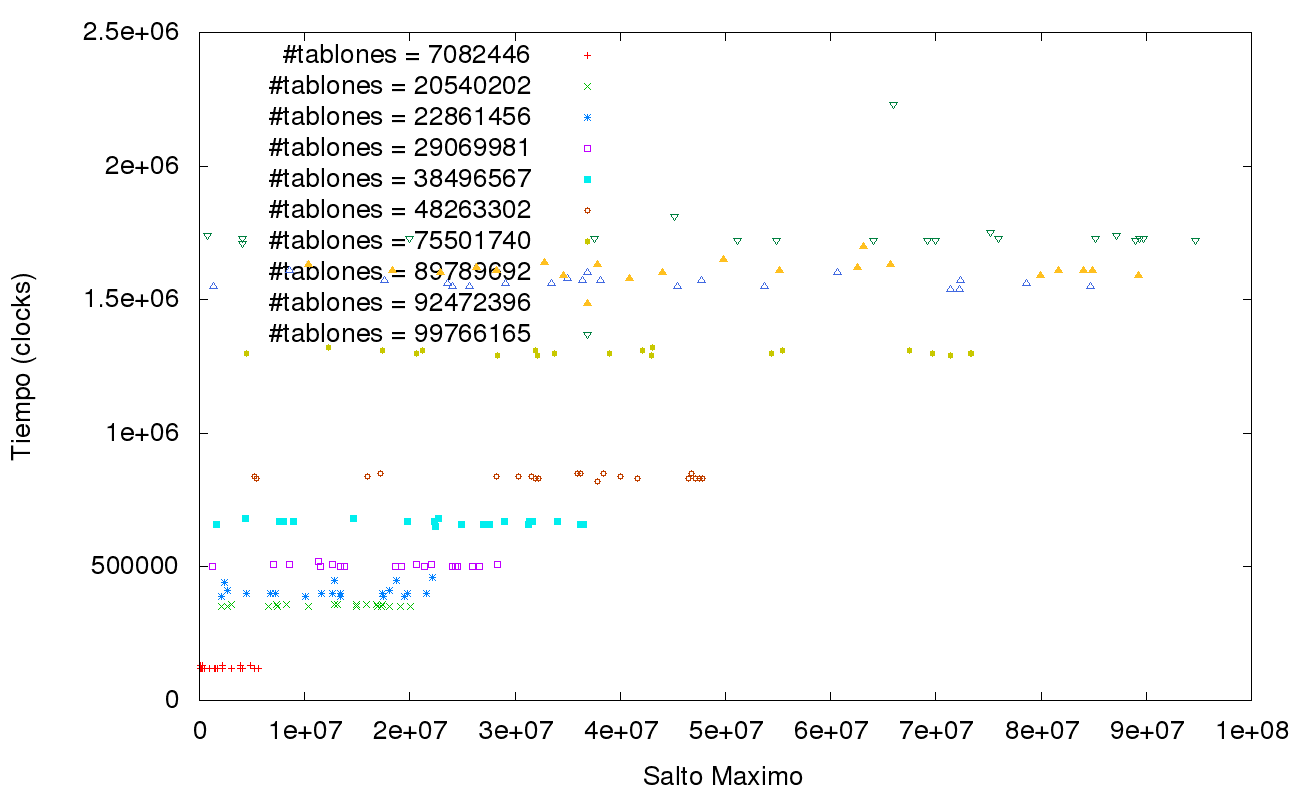
\includegraphics[scale=.45]{./imagenes/ej1_testSaltoMaximo.png}
\caption{Gr\'afico de tiempo en funci\'on del salto m\'aximo.}
\end{center}
\end{figure}

